\subsection{Artificially Intelligent Agents} \label{sec:aias}
    As noted by \citet{Tripp2011-rx}, intelligent technology spans a wide spectrum of capabilities. With regards to autonomous systems, one might consider anything from a thermostat, to HAL 9000. While the main interest of the author is geared towards the capability of humans to trust `advanced' technology, for the purposes of this survey we will take a more holistic view and use the term \textit{Artificially Intelligent Agent (AIA)} to encompass a broad range of technologies that can be considered `automatic' by some sense of the word. This is done in order to provide generally applicable definitions.

    It is widely accepted that an artificial intelligence needs to possess at least some of the capabilities shown in Figure~\ref{fig:AIcapabilities}~\cite{Russell2010-wv,Nilsson2009-rp,Luger2008-vf}\footnote{This group of capabilities would generally be accepted in the AI community, although some argue that it is  necessary to add other categories like creativity, and social intelligence~\cite{Duch2007-oi,Tao2005-kh}. Of course this set of attributes is not universally accepted, and is still being refined.}. The following simple definitions will help to ground further discussion in the paper:

    \begin{description}
        \item [Reasoning:] The ability to solve problems, and make conclusions.
        \item [Knowledge Representation:] The ability to internally represent knowledge of information that has been learned.
        \item [Planning:] The ability to make a plan in order to accomplish a goal within an environment.
        \item [Learning:] The ability to learn from experience and data.
        \item [Perception:] The ability to use different sensors to perceive the surrounding environment.
        \item [Motion/Manipulation:] The ability to move within an environment and manipulate parts of it.
        \item [Interaction:] The ability to interact with other intelligent agents. For communicating with humans this could involve some type of natural language interface.
    \end{description}

	\begin{figure}[htbp]
    	\centering
     	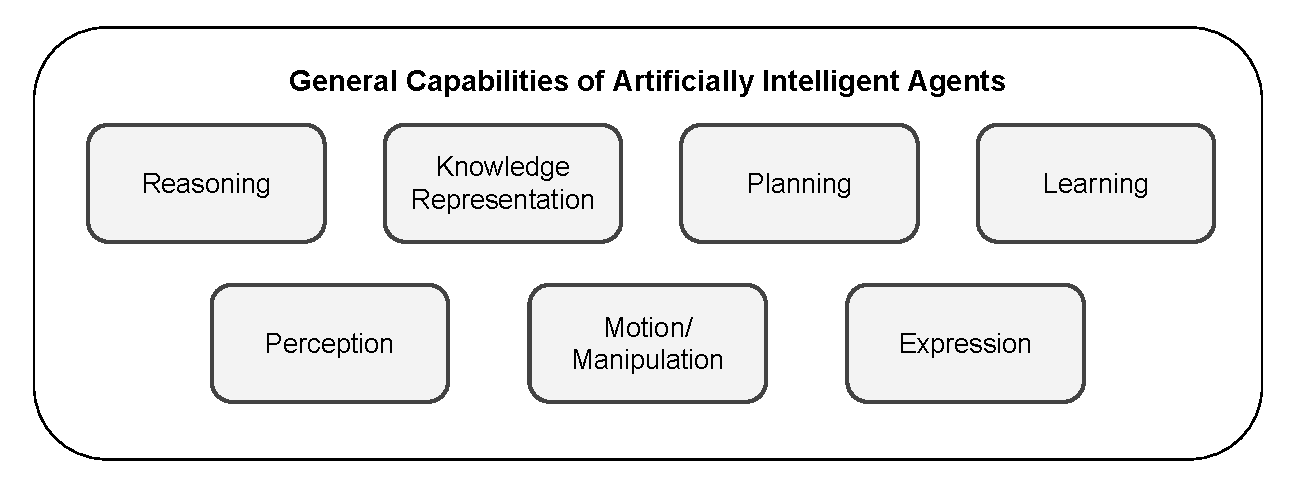
\includegraphics[width=0.7\textwidth]{Figures/AI_capabilities}
    	\caption{List of the capabilities of an artificial general intelligence. In this paper an AI is defined as a system that possesses at least one of the capabilities illustrated. AIA capabilities are the sources of assurances.}
        \label{fig:AIcapabilities}
    \end{figure}

    It should be noted that the categories are not clearly separable; for instance, where does the capability to `plan' end and `reasoning' begin? Similar questions could be asked of the other capabilities. Regardless, these capability categories are conceptually useful in defining an AIA:
    
    \begin{description}
        \item[Artificially Intelligent Agent (AIA):] an agent that acts on a goal (internally or externally generated), and possesses, to some extent, at least one of the capabilities shown in Figure~\ref{fig:AIcapabilities}.
    \end{description}

    Of course, with such a broad definition, there will also be a broad range of different AIAs. For the purposes of this discussion, is most useful to classify that range along two axes: scope, and adaptability. Scope refers to the range of possible applications of the AIA: does it have a certain specific application, or can it be used in many different applications? Agents with narrow scope are more specialized, while those with a broad scope can be applied in more diverse applications. Adaptability refers to the ability of the AIA to become better at executing its goal over time. Low adaptability has often been associated with `weak AI' whereas high adaptability is often associated with `strong AI'. Figure~\ref{fig:StrongWeak} is a depiction of these two axes, and where some AIAs (real and fictitious) might fall in that space.

	\begin{figure}[htbp]
    	\centering
     	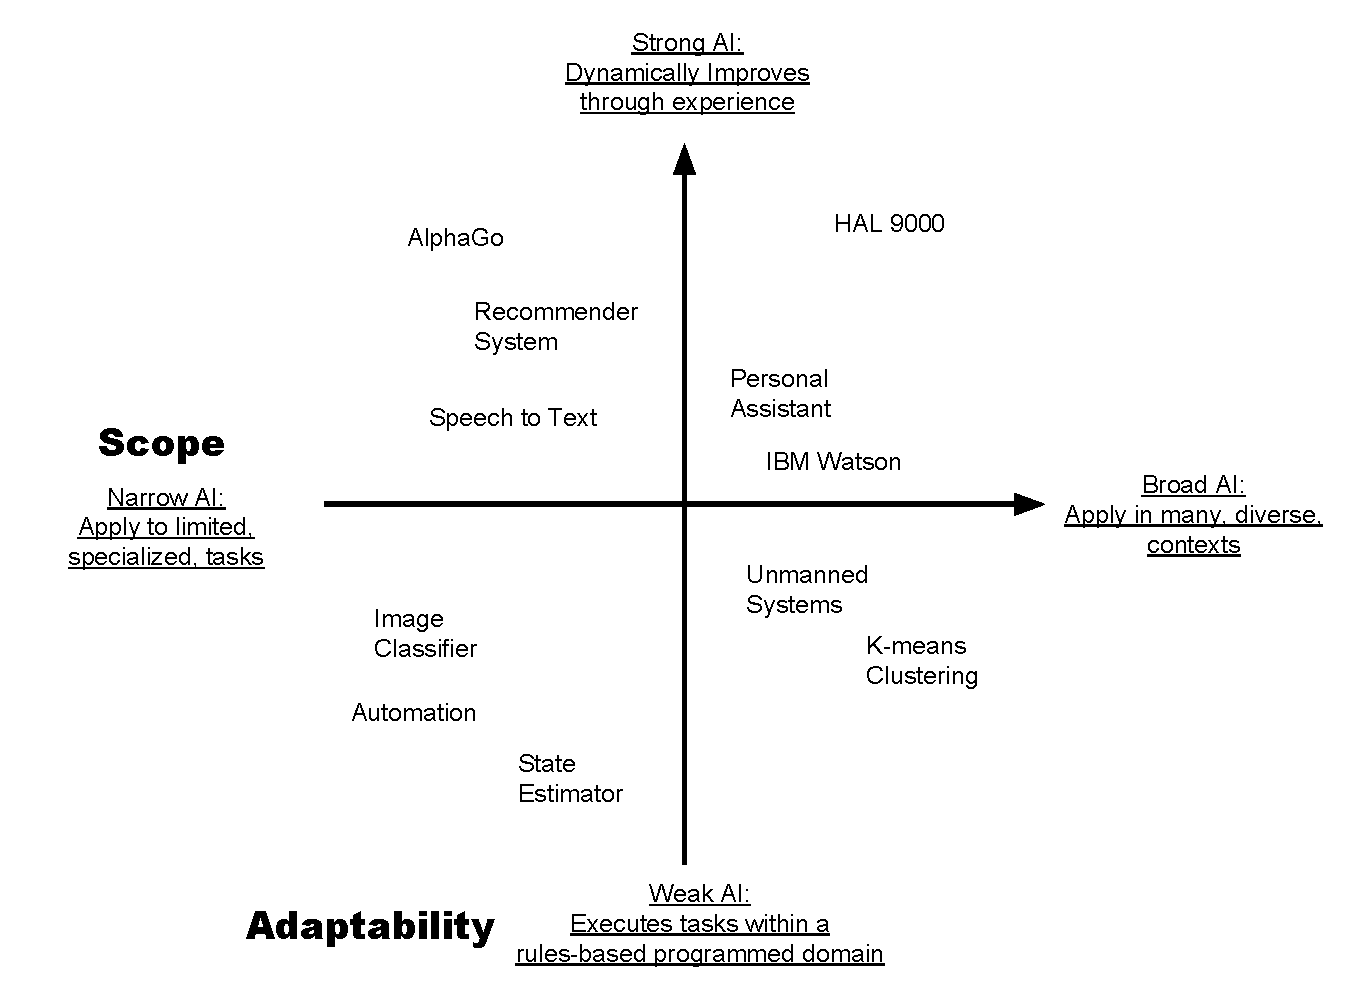
\includegraphics[width=0.7\textwidth]{Figures/strong_weak_narrow_broad.pdf}
    	\caption{Illustration of the range of systems encompassed by the AIA definition. Horizontal axis reflects the scope of the AIA, the vertical axis reflects the adaptability of the AIA.}
        \label{fig:StrongWeak}
    \end{figure}

  Arguably, we might just as well use the term `artificial intelligence' (AI) instead of AIA. However, `AI' carries too much ambiguity (in its fullest meaning, it would possess all capabilities from Figure~\ref{fig:AIcapabilities}, and more). AIA allows the broad inclusion of \emph{any} system in the adaptability/scope plane. %%--nra: already said this above: Figure~\ref{fig:StrongWeak} shows some examples of AIAs and their places on the plane. %%%
To make sure the point is clear, the research discipline called machine learning (ML) is a subset of the AI research landscape. Individual ML algorithms might be thought of as being a narrowly scoped AI that is contained within only one of the AIA capabilities. As some examples, consider the following systems and the capabilities that they possess.

    \begin{enumerate}
         \item An autonomous bottle capping machine can \textbf{perceive} bottles, and \textbf{move} mechanical parts to place caps on them;
         \item An unmanned aerial system (UAS) might possess the ability to \textbf{plan} missions, \textbf{perceive} an agent vehicle's location, and execute \textbf{motion} of its components to carry out a plan; 
         \item A virtual personal assistant might be capable of \textbf{interacting} with a user, \textbf{learning} the user's preferences, and \textbf{reasoning} about what assistance the user needs;
         \item An image classifier might possess the capability to \textbf{learn} image classes from labeled examples and predict the class of never-before-seen new images.
     \end{enumerate}

    One might also question the need to define AIAs in the first place. This is to aid in the search for and understanding of assurances. As will be shown later, different methods of assurance can be found over the entire range of AIAs, so that an automation system such as a bottle capping machine might be able to use similar assurances -- or more generally, similar principles of assurance -- as might a self-driving car, and vice-versa. The capabilities of AIAs (Fig.~\ref{fig:AIcapabilities}) are the sources of assurances; in other words, assurances cannot exist without some grounding set of AIA capabilities. 

This definition, while broad, is still useful because it encompasses many of the systems that are typically described as `artificially intelligent'. More importantly, many of the assurances that exist for the simplest AIAs (e.g. chi-square consistency tests for a Kalman filter state estimator) can be adapted/generalized for use in more advanced AIAs. 
In other words, the definition of AIAs sets an appropriate scope for the bodies of research that are likely to have investigated assurances and assurance principles that can be generalized/extended to any intelligent computing system. The definition of AIAs and their range of capabilities also helps to understand and establish what kinds of assurances might be needed in future systems. For example, assurances from an AIA that can only carry out planning tasks will probably differ in design and/or application from assurances from an AIA that can only carry out perception tasks. 
